\section{Accounting for the variability in gene copy number during the cell
cycle} \label{supp_multi_gene}

(Note: The Python code used for the calculations presented in this section can
be found in the
\href{https://www.rpgroup.caltech.edu/chann_cap/src/theory/html/moment_dynamics_cell_division.html}{following
link} as an anotated Jupter notebook)

When growing in rich media, bacteria can double every $\approx$ 20 minutes.
With two replication forks each traveling at $\approx$ 1000 bp per second, and
a genome of $\approx$ 5 Mbp for {\it E. coli} \cite{Moran2010}, a cell would
need $\approx$ 40 minutes to replicate its genome. The apparent paradox  of
growth rates faster than one division per 40 minutes is solved by the fact that
cells have multiple replisomes, i.e. molecular machines that replicate the
genome running in parallel. Cells can have up to 8 copies of the genome being
replicated simultaneously depending on the growth rate \cite{Bremer1996}.

This observation implies that during the cell cycle gene copy number varies.
This variation depends on the growth rate and the relative position of the gene
with respect to the replication origin, having genes close to the replication
origin spending more time with multiple copies compare to genes closer to the
replication termination site. This change in gene dosage has a direct effect on
the cell-to-cell variability in gene expression \cite{Jones2014a,
Peterson2015}.

\subsection{Numerical integration of moment equations}

For our specific locus ({\it galK}) and a doubling time of $\approx$ 100 min
for our experimental conditions, cells have on average 1.4 copies of the
reporter gene during the cell cycle. What this means is that cells spend 60\%
of the time having one copy of the gene and 40\% of the time with two copies.
To account for this variability in gene copy number across the cell cycle we
numerically integrate the moment equations derived in \siref{supp_moments} for
a time $t = [0, t_s]$ with an mRNA production rate $r_m$, where $t_s$ is the
time point at which the replication fork reaches our specific locus. For the
remaining time before the cell division $t = [t_s, t_d]$ that the cell spends
with two promoters, we assume that the only parameter that changes is the mRNA
production rate from $r_m$ to $2 r_m$. This simplifying assumption ignores
potential changes in protein translation rate $r_p$ or changes in the repressor
copy number that would be reflected in changes on the repressor on rate
$\kron$.

\subsubsection{Computing distribution moments after cell division}

We have already solved a general form for the dynamics of the moments of the
distribution, i.e. we wrote differential equations for the moments ${d\ee{m^x
p^y}\over dt}$. Given that we know all parameters for our model we can simply
integrate these equations numerically to compute how the moments of the
distribution evolve as cells progress through their cell cycle. Once the cell
reaches a time $t_d$ when is going to divide the mRNA and proteins that we are
interested in undergo a binomial partitioning between the two daughter cells.
In other words, each molecule flips a coin and decides whether to go to either
daughter. The question then becomes given that we have a value for the moment
$\ee{m^x p^y}_{t_d}$ at a time before the cell division, what would the value
of this moment be after the cell division takes place $\ee{m^x p^y}_{t_o}$?

The probability distribution of mRNA and protein after the cell division
$P_{t_o}(m, p)$ must satisfy
\begin{equation}
  P_{t_o}(m, p) = \sum_{m'=m}^\infty \sum_{p'=p}^\infty 
                  P(m, p \mid m', p') P_{t_d}(m', p'),
\label{eq_dist_post_div}
\end{equation}
where we are summing over all the possibilities of having $m'$ mRNA and $p'$
proteins before cell division. Note that the sums start at $m$ and $p$; this is
because for a cell to have these copy numbers before cell division it is a
requirement that the mother cell had at least such copy number since we are not
assuming that there is any production at the instantaneous cell division time.
Since we assume that the partition of mRNA is independent from the partition of
protein, the conditional probability $P(m, p \mid m', p')$ is simply given by a
product of two binomial distributions, one for the mRNA and one for the
protein, i.e.
\begin{equation}
P(m, p \mid m', p') = {m' \choose m} \left( {1 \over 2} \right)^{m'} \cdot
                      {p' \choose p} \left( {1 \over 2} \right)^{p'}.
\label{eq_binom_prod}
\end{equation}
Because of these product of binomial probabilities are allowed to extend the
sum from
\eref{eq_dist_post_div} to start at $m'=0$ and $p'=0$ as
\begin{equation}
  P_{t_o}(m, p) = \sum_{m'=0}^\infty \sum_{p'=0}^\infty 
                  P(m, p \mid m', p') P_{t_d}(m', p'),
\end{equation}
since the product of the binomial distributions in \eref{eq_binom_prod} is zero
for all $m' < m$ and/or $p' < 0$. So from now on in this section we will assume
that a sum of the form $\sum_x \equiv \sum_{x=0}^\infty$ to simplify notation.

We can then compute the distribution moments after the cell division $\ee{m^x
p^y}_{t_o}$ as
\begin{equation}
\ee{m^x p^y}_{t_o} = \sum_m \sum_p m^x p^y P_{t_o}(m, p),
\end{equation}
for all $x, y \in \mathbb{N}$. Substituting \eref{eq_dist_post_div} results in
\begin{equation}
\ee{m^x p^y}_{t_o} = \sum_m \sum_p m^x p^y
\sum_{m'} \sum_{p'} P(m, p \mid m', p') P_{t_d}(m', p').
\end{equation}
We can rearrange the sums to be 
\begin{equation}
\ee{m^x p^y}_{t_o} = \sum_{m'} \sum_{p'} P_{t_d}(m', p')
                     \sum_m \sum_p m^x p^y P(m, p \mid m', p').
\end{equation}
The fact that \eref{eq_binom_prod} is the product of two independent events
allows us to rewrite the joint probability $P(m, p \mid m', p')$ as
\begin{equation}
P(m, p \mid m', p') = P(m \mid m') \cdot P(p \mid p').
\end{equation}
With this we can then write the moment $\ee{m^x p^y}_{t_o}$ as
\begin{equation}
\ee{m^x p^y}_{t_o} = \sum_{m'} \sum_{p'} P_{t_d}(m', p')
                     \sum_m  m^x  P(m \mid m')
                     \sum_p p^y P(p \mid p').
\end{equation}
Notice that both terms summing over $m$ and over $p$ are the conditional
expected values, i.e.
\begin{equation}
\sum_z  z^x  P(z \mid z') \equiv \ee{z^x \mid z'}, \; 
{\text{ for } z\in \{m, p \}}.
\end{equation}
These conditional expected values are the expected values of a binomial random
variable $z \sim \text{Bin}(z', 1/2)$, which can be easily computed as we will
show later in this section. We then rewrite the expected values after the cell
division in terms of these moments of a binomial distribution
\begin{equation}
\ee{m^x p^y}_{t_o} = \sum_{m'} \sum_{p'} \ee{m^x \mid m'} \ee{p^y \mid p'} 
                     P_{t_d}(m', p').
  \label{eq_general_binom_mom}
\end{equation}

To see how this general formula for the moments after the cell division works
let's compute the mean protein per cell after the cell division $\ee{p}_{t_o}$.
That is setting $x = 0$, and $y = 1$. This results in
\begin{equation}
\ee{p}_{t_o} = \sum_{m'} \sum_{p'} \ee{m^0 \mid m'} \ee{p \mid p'} 
               P_{t_d}(m', p').
\end{equation}
The zeroth moment $\ee{m^0 \mid m'}$ by definition must be one since we have
\begin{equation}
\ee{m^0 \mid m'} = \sum_m m^0 P(m \mid m') = \sum_m P(m \mid m') = 1,
\end{equation}
since the probability distribution must be normalized. This leaves us then with
\begin{equation}
\ee{p}_{t_o} = \sum_{m'} \sum_{p'} P_{t_d}(m', p') \ee{p \mid p'}.
\end{equation}
If we take the sum over $m'$ we simply compute the marginal probability
distribution $\sum_{m'} P_{t_d}(m', p') = P_{t_d}(p')$, then we have
\begin{equation}
\ee{p}_{t_o} = \sum_{p'} \ee{p \mid p'} P_{t_d}(p').
\end{equation}
For the particular case of the first moment of the binomial distribution with
parameters $p'$ and $1/2$ we know that
\begin{equation}
\ee{p \mid p'} = {p' \over 2}.
\end{equation}
Therefore the moment after division is equal to
\begin{equation}
\ee{p}_{t_o} = \sum_{p'} {p' \over 2} P_{t_d}(p')
             = {1 \over 2} \sum_{p'} p' P_{t_d}(p').
\end{equation}
Notice that this is just 1/2 of the expected value of $p'$ averaging over the
distribution prior to cell division, i.e.
\begin{equation}
\ee{p}_{t_o} = {\ee{p'}_{t_d} \over 2},
\end{equation}
where $\ee{\cdot}_{t_d}$ highlights that is the moment of the distribution
prior to the cell division. This result makes perfect sense. What this is
saying is that the mean protein copy number right after the cell divides is
half of the mean protein copy number just before the cell division. That is
exactly we would expect. So in principle to know the first moment of either the
mRNA distribution $\ee{m}_{t_o}$ or the protein distribution $\ee{m}_{t_o}$
right after cell division it suffices to multiply the moments before the cell
division $\ee{m}_{t_d}$ or $\ee{p}_{t_d}$ by 1/2. Let's now explore how this
generalizes to any other moment $\ee{m^x p^y}_{t_o}$.

\subsubsection{Computing the moments of a binomial distribution}

The result from last section was dependent on us knowing the functional form of
the first moment of the binomial distribution. For higher moments we need some
systematic way to compute such moments. Luckily for us we can do so by using
the so-called moment generating function (MGF). The MGF of a random variable
$X$ is defined as
\begin{equation}
M_X(t) = \ee{e^{tX}},
\end{equation}
where $t$ is a dummy variable. Once we know the MGF we can obtain any moment of
the distribution by simply computing
\begin{equation}
  \ee{X^n} = \left. {d^n \over dt^n} M_X(t) \right\vert_{t=0},
  \label{eq_mgf_def}
\end{equation}
i.e. taking the $n$-th derivative of the MGF returns the $n$-th moment of the
distribution. For the particular case of the binomial distribution $X \sim
\text{Bin}(N, q)$ it can be shown that the MGF is of the form
\begin{equation}
M_X(t) = \left[ (1 - q) + qe^{t} \right]^N.
\end{equation}
As an example let's compute the first moment of this binomially distributed
variable. For this, the first derivative of the MGF results in
\begin{equation}
  {d M_X(t) \over dt} = N [(1 - q) + qe^t]^{N - 1} q e^t.
\end{equation}
We just need to follow \eref{eq_mgf_def} and set $t = 0$ to obtain the first
moment
\begin{equation}
  \left. {d M_X(t) \over dt} \right\vert_{t=0} = N q,
  \label{eq_mgf_mean}
\end{equation}
which is exactly the expected value of a binomially distributed random
variable.

So according to \eref{eq_general_binom_mom} to compute any moment $\ee{m^x
p^y}$ after cell division we can just take the $x$-th derivative and the $y$-th
derivative of the binomial MGF to obtain $\ee{m^x \mid m'}$ and $\ee{p^y \mid
p'}$, respectively, and take the expected value of the result. Let's follow on
detail the specific case for the moment $\ee{m p}$. When computing the moment
after cell division $\ee{mp}_{t_o}$ which is of
the form
\begin{equation}
\ee{mp}_{t_o} = \sum_{m'} \sum{p'} \ee{m \mid m'} \ee{p \mid p'} 
                P_{t_d}(m', p'),
\end{equation}
the product $\ee{m \mid m'} \ee{p \mid p'}$ is then
\begin{equation}
\ee{m \mid m'} \ee{p \mid p'} = {m' \over 2} \cdot {p' \over 2},
\end{equation}
where we used the result in \eref{eq_mgf_mean}, substituting $m$ and $p$ for
$X$, respectively, and $q$ for 1/2. Substituting this result into the moment
gives
\begin{equation}
\ee{mp}_{t_o} = \sum_{m'} \sum_{p'} {m' p' \over 4} P_{t_d}(m', p') 
              = {\ee{m' p'}_{t_d} \over 4}.
\end{equation}
Therefore to compute the moment after cell division $\ee{mp}_{t_o}$ we simply
have to divide by 4 the corresponding equivalent moment before the cell
division. 

Not all moments after cell division depend only on the equivalent moment before
cell division. For example if we compute the third moment of the protein
distribution $\ee{p^3}_{t_o}$, we find
\begin{equation}
  \ee{p^3}_{t_o} = {\ee{p^3}_{t_d} \over 8} + {3 \ee{p^2}_{t_d} \over 8}.
\end{equation}
So for this particular case the third moment of the protein distribution
depends on the third moment and the second moment before the cell division. In
general all moments after cell division $\ee{m^x p^y}_{t_o}$ linearly depend on
moments before cell division. Furthermore, there is ``moment closure'' for this
specific case in the sense that all moments after cell division depend on lower
moments before cell division. To generalize these results to all the moments
computed in this work let us then define a vector to collect all moments before
the cell division up the $\ee{m^x p^y}_{t_d}$ moment, i.e.
\begin{equation}
\bb{\ee{m^x p^y}}_{t_d} = \left(
\ee{m^0 p^0}_{t_d}, \ee{m^1}_{t_d}, \ldots , \ee{m^x p^y}_{t_d}
\right).
\end{equation}
Then any moment after cell division $\ee{m^{x'} p^{y'}}_{t_o}$ for $x' \leq x$ and $y' \leq y$ can be computed as
$$
\ee{m^{x'} p^{y'}}_{t_o} = \bb{z}_{x'y'} \cdot \bb{\ee{m^x p^y}}_{t_d},
$$
where we define the vector $\bb{z}_{x'y'}$ as the vector containing all the coefficients that we obtain with the product of the two binomial distributions.
For example for the case of the third protein moment $\ee{p^3}_{t_o}$ the vector $\bb{z}_{x'y'}$ would have zeros for all entries except for the corresponding entry for $\ee{p^2}_{t_d}$ and for $\ee{p^3}_{t_d}$, where it would have $3/8$ and $1/8$ accordingly.

If we want then to compute all the moments after the cell division up to
$\ee{m^x p^y}_{t_o}$ let us define an equivalent vector
\begin{equation}
\bb{\ee{m^x p^y}}_{t_o} = \left(
\ee{m^0 p^0}_{t_o}, \ee{m^1}_{t_o}, \ldots , \ee{m^x p^y}_{t_o}
\right).
\end{equation}
Then we need to build a square matrix $\bb{Z}$ such that each row of the matrix
contains the corresponding vector $\bb{z}_{x' y'}$ for each of the moments.
Having this matrix we would simply compute the moments after the cell division
as
\begin{equation}
\bb{\ee{m^x p^x}}_{t_o} = \bb{Z} \cdot \bb{\ee{m^x p^x}}_{t_d}.
\end{equation}
In other words, matrix $\bb{Z}$ will contain all the coefficients that we need
to multiply by the moments before the cell division in order to obtain the
moments after cell division. Matrix $\bb{Z}$ was then generated automatically
using Python's analytical math library
\href{https://www.sympy.org/en/index.html}{\texttt{sympy}}.

\fref{sfig_first_mom_cycles} (adapted from \fref{fig3_cell_cycle}(B)) shows how
the first moment of both mRNA and protein changes over several cell cycles. The
mRNA quickly relaxes to the steady state corresponding to the parameters for
both a single and two promoter copies. This is expected since the parameters
for the mRNA production were determined in the first place under this
assumption (See \siref{supp_model}). We note that there is no apparent delay
before reaching steady state of the mean mRNA count after the cell divides.
This is because the mean mRNA count for the two promoters copies  state is
exactly twice the expected mRNA count for the single promoter state (See
\siref{supp_model}). Therefore once the mean mRNA count is halved after the
cell division, it is already at the steady state value for the single promoter
case. On the other hand, given that the relaxation time to steady state is
determined by the degradation rate, the mean protein count does not reach its
corresponding steady state value for either promoter copy number state.
Interestingly once a couple of cell cycles have passed the first moment has a
repetitive trajectory over cell cycles. We have observed this experimentally by
tracking cells as they grow under the microscope. Comparing cells at the
beginning of the cell cycle with the daughter cells that appear after cell
division shown that on average all cells have the same amount of protein at the
beginning of the cell cycle (See Fig. 18 of \cite{Phillips2019}), suggesting
that these dynamical steady state takes place \textit{in vivo}.

\begin{figure}[h!]
	\centering 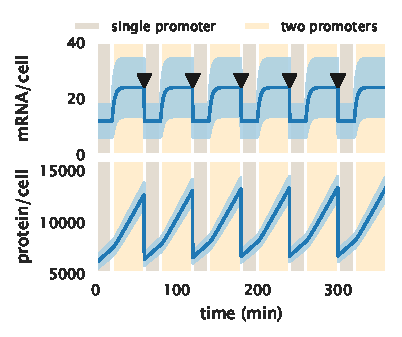
\includegraphics
  {../fig/main/fig03B.pdf}
	\caption{\textbf{First and second moment dynamics over cell the cell cycle.}
	Mean $\pm$ standard deviation mRNA (upper panel) and mean $\pm$ standard
	deviation protein copy number (lower panel) as the cell cycle progresses. The
	dark shaded region delimits the fraction of the cell cycle that cells spend
	with  a single copy of the promoter. The light shaded region delimits the
	fraction of the cell cycle that cells spend with two copies of the promoter.
	For a 100 min doubling time at the {\it galK} locus cells spend 60\% of the
	time with one copy of the promoter and the rest with two copies.}
  \label{sfig_first_mom_cycles}
\end{figure}

In principle when measuring gene expression levels experimentally from an
asynchronous culture, cells are sampled from any time point across their
individual cell cycles. This means that the moments determined experimentally
correspond to an average over the cell cycle. In the following section we
discuss how to account for the fact that cells are not uniformly distributed
across the cell cycle in order to compute these averages.

\subsection{Exponentially distributed ages}

As mentioned in \siref{supp_param_inference}, cells in exponential growth have
exponentially distributed ages across the cell cycle, having more young cells
compared to old ones. Specifically the probability of a cell being at any time
point in the cell cycle is given by \cite{Powell1956}
\begin{equation}
  P(a) = (\ln 2) \cdot 2^{1 - a},
  \label{seq_age_prob}
\end{equation}
where $a \in [0, 1]$ is the stage of the cell cycle, with $a = 0$ being the
start of the cycle and $a = 1$ being the cell division. In
\siref{supp_cell_age_dist} we reproduce this derivation. It is a surprising
result, but can be intuitively thought as follows: If the culture is growing
exponentially, that means that all the time there is an increasing number of
cells. That means for example that if in a time interval $\Delta t$ $N$ ``old''
cells divided, these produced $2N$ ``young'' cells. So at any point there is
always more younger than older cells.

Our numerical integration of the moment equations gave us a time evolution of
the moments as cells progress through the cell cycle. Since experimentally we
sample asynchronous cells that follow \eref{seq_age_prob}, each time point along
the moment dynamic must be weighted by the probability of having sampled a cell
at such specific time point of the cell cycle. Without loss of generality let's
focus on the first mRNA moment $\ee{m(t)}$ (the same can be applied to all other
moments). As mentioned before, in order to calculate the first moment across the
entire cell cycle we must weigh each time point by the corresponding probability
that a cell is found in such point of its cell cycle. This translates to
computing the integral
\begin{equation}
  \ee{m}_c = \int_{\text{beginning cell cycle}}^{\text{end cell cycle}}
                       \ee{m(t)} P(t) dt,
\end{equation}
where $\ee{m}_c$ is the mean mRNA copy number averaged over the entire cell
cycle trajectory, and $P(t)$ is the probability of a cell being at a time $t$ of
its cell cycle.

If we set the time in units of the cell cycle length we can use
\eref{seq_age_prob} and compute instead
\begin{equation}
  \ee{m} = \int_0^1 \ee{m(a)} P(a) da,
  \label{seq_moment_avg}
\end{equation}
where $P(a)$ is given by \eref{seq_age_prob}.

What \eref{seq_moment_avg} implies is that in order to compute the first moment
(or any moment of the distribution) we must weigh each point in the moment
dynamics by the corresponding probability of a cell being at that point along
its cell cycle. That is why when computing a moment we take the time trajectory
of a single cell cycle as the ones shown in \fref{sfig_first_mom_cycles} and
compute the average using \eref{seq_age_prob} to weigh each time point. We
perform this integral numerically for all moments using Simpson's rule.

\subsection{Reproducing the equilibrium picture}

Given the large variability of the first moments depicted in
\fref{sfig_first_mom_cycles} it is worth considering why a simplistic
equilibrium picture has shown to be very successful in predicting the mean
expression level under diverse conditions \cite{Garcia2011c, Brewster2014,
Barnes2019, Razo-Mejia2018}. In this section we compare the simple repression
thermodynamic model with this dynamical picture of the cell cycle. But before
diving into this comparison, it is worth recapping the assumptions that go into
the equilibrium model.

\subsubsection{Steady state under the thermodynamic model}

Given the construction of the thermodynamic model of gene regulation for which
the probability of the promoter microstates rather than the probability of mRNA
or protein counts is accounted for,  we are only allowed to describe the
dynamics of the first moment using this theoretical framework
\cite{Phillips2015}. Again let's only focus on the mRNA first moment $\ee{m}$.
The same principles apply if we consider the protein first moment. We can write
a dynamical system of the form
\begin{equation}
  \dt{\ee{m}} = r_m \cdot \pbound - \gm \ee{m},
\end{equation}
where as before $r_m$ and $\gm$ are the mRNA production and degradation rates
respectively, and $\pbound$ is the probability of finding the RNAP bound to the
promoter \cite{Bintu2005a}. This dynamical system is predicted to have a single
stable fixed point that we can find by computing the steady state. When we solve
for the mean mRNA copy number at steady state $\ee{m}_{ss}$ we find
\begin{equation}
  \ee{m}_{ss} = {r_m \over \gm} \pbound.
\end{equation}

Since we assume that the only effect that the repressor has over the regulation
of the promoter is exclusion of the RNAP from binding to the promoter, we assume
that only $\pbound$ depends on the repressor copy number $R$. Therefore when
computing the fold-change in gene expression we  are left with
\begin{equation}
  \foldchange = {\ee{m (R \neq 0)}_{ss} \over \ee{m (R = 0)}_{ss}}
              = {\pbound (R \neq 0) \over \pbound (R = 0)}.
\end{equation}
As derived in \cite{Garcia2011c} this can be written in the language of
equilibrium statistical mechanics as
\begin{equation}
  \foldchange = \left(1 + {R \over \Nns}e^{-\beta \eR}  \right)^{-1},
  \label{seq_fold_change_thermo}
\end{equation}
where $\beta \equiv (k_BT)^{-1}$, $\eR$ is the repressor-DNA binding energy, and
$\Nns$ is the number of non-specific binding sites where the repressor can bind.

To arrive at \eref{seq_fold_change_thermo} we ignore the physiological changes
that occur during the cell cycle; one of the most important being the
variability in gene copy number that we are exploring in this section. It is
therefore worth thinking about whether or not the dynamical picture exemplified
in \fref{sfig_first_mom_cycles} can be reconciled with the predictions made by
\eref{seq_fold_change_thermo} both at the mRNA and protein level.

\fref{sfig_lacI_titration} compares the predictions of both theoretical
frameworks for varying repressor copy numbers and repressor-DNA affinities. The
solid lines are directly computed from \eref{seq_fold_change_thermo}. The hollow
triangles and the solid circles, represent the fold-change in mRNA and protein
respectively as computed from the moment dynamics. To compute the fold-change
from the kinetic picture we first numerically integrate the moment dynamics for
both the two- and the three-state promoter (See \fref{sfig_first_mom_cycles} for
the unregulated case) and then average the time series accounting for the
probability of cells being sampled at each stage of the cell cycle as defined in
\eref{seq_moment_avg}. The small systematic deviations between both models come
partly from the simplifying assumption that the repressor copy number, and
therefore the repressor on rate $\kron$ remains constant during the cell cycle.
In principle the gene producing the repressor protein itself is also subjected
to the same duplication during the cell cycle, changing therefore the mean
repressor copy number for both stages.

\begin{figure}[h!]
	\centering \includegraphics
  {../fig/moment_dynamics_numeric/lacI_titration.pdf}
	\caption{\textbf{Comparison of the equilibrium and kinetic reressor titration
	predictions.} The equilibrium model (solid lines) and the kinetic model with
	variation over the cell cycle (solid circles and white triangles) predictions
	are compared for varying repressor copy numbers and operator binding energy.
	The equilibrium model is directly computed from \eref{seq_fold_change_thermo}
	while the kinetic model is computed by numerically integrating the moment
	equations over several cell cycles, and then averaging over the extent of the
	cell cycle as defined in \eref{seq_moment_avg}.}
  \label{sfig_lacI_titration}
\end{figure}

For completeness \fref{sfig_IPTG_titration} compares the kinetic and equilibrium
models for the extended model of \cite{Razo-Mejia2018} in which the inducer
concentration enters into the equation. The solid line is directly computed from
Eq. 5 of \cite{Razo-Mejia2018}. The hollow triangles and solid points follow the
same procedure as for \fref{sfig_lacI_titration}, where the only effect that the
inducer is assume to have in the kinetics is an effective change in the number
of active repressors, affecting therefore $\kron$.

\begin{figure}[h!]
	\centering \includegraphics
  {../fig/moment_dynamics_numeric/IPTG_titration.pdf}
	\caption{\textbf{Comparison of the equilibrium and kinetic inducer titration
	predictions.} The equilibrium model (solid lines) and the kinetic model with
	variation over the cell cycle (solid circles and white triangles) predictions
	are compared for varying repressor copy numbers and inducer concentrations.
	The equilibrium model is directly computed as Eq. 5 of reference
	\cite{Razo-Mejia2018} with repressor-DNA binding energy $\eR = -13.5 \; k_BT$
	while the kinetic model is computed by numerically integrating the moment
	dynamics over several cell cycles, and then averaging over the extent of a
	single cell cycle as defined in \eref{seq_moment_avg}.}
  \label{sfig_IPTG_titration}
\end{figure}

\subsection{Comparison between single- and multi-promoter kinetic model}

After these calculations it is worth questioning whether the inclusion of this
change in gene dosage is drastically different with respect to
the simpler picture of a kinetic model that ignores the gene copy number
variability during the cell cycle. To this end we systematically computed the
average moments for varying repressor copy number and repressor-DNA affinities.
We then compare these results with the moments obtained from a single-promoter
model and their corresponding parameters. The derivation of the steady-state
moments of the distribution for the single-promoter model are detailed in
\siref{supp_moments}.

\fref{sfig_lacI_titration} and \fref{sfig_IPTG_titration} both suggest that
since the dynamic multi-promoter model can reproduce the results of the
equilibrium model at the first moment level it must then also be able to
reproduce the results of the single-promoter model at this level (See
\siref{supp_param_inference}). The interesting comparison comes with higher
moments. A useful metric to consider for gene expression variability is the
noise in gene expression \cite{Shahrezaei2008}. This quantity, defined as the
standard deviation divided by the mean, is a dimensionless metric of how much
variability there is with respect to the mean of a distribution. As we will show
below this quantity differs from the also commonly used metric known as the Fano
factor (variance / mean) in the sense that for experimentally determined
expression levels in fluorescent arbitrary units, the noise is a dimensionless
quantity while the Fano factor is not.

\fref{sfig_noise_comparison} shows the comparison of the predicted protein noise
between  the single- (dashed lines) and the multi-promoter model (solid lines)
for different operators and repressor copy numbers. A striking difference
between both is that the single-promoter model predicts that as the inducer
concentration increases, the standard deviation grows much slower than the mean,
giving a very small noise. In comparison the multi-promoter model has a much
higher floor for the lowest value of the noise, reflecting the expected result
that the variability in gene copy number across the cell cycle should increase
the cell-to-cell variability in gene expression \cite{Peterson2015, Jones2014a}

\begin{figure}[h!]
	\centering \includegraphics
  {../fig/moment_dynamics_numeric/noise_comparison.pdf}
	\caption{\textbf{Comparison of the predicted protein noise between a single-
	and a multi-promoter kinetic model.} Comparison of the noise
	(standard deviation/mean) between a kinetic model that considers a single
	promoter at all times (dashed line) and the multi-promoter model developed
	in this section (solid line) for different repressor operators. (A) Operator
	O1,  $\eR = -15.3 \; k_BT$, (B) O2, $\eR = -13.9 \; k_BT$, (C) O3, $\eR =
	-9.7 \; k_BT$}
  \label{sfig_noise_comparison}
\end{figure}

\subsection{Comparison with experimental data}\label{supp_theory_vs_data_mom}

Having shown that the kinetic model presented in this section can reproduce the
results from the equilibrium picture at the mean level (See
\fref{sfig_lacI_titration} and \fref{sfig_IPTG_titration}), but changes the
prediction for the cell-to-cell variability as quantified by the noise
(See \fref{sfig_noise_comparison}), we can assess whether or not this model is
able to predict experimental measurements of the noise. For this we take the
single cell intensity measurements (See Methods) to compute the noise at the
protein level.

As mentioned before this metric differs from the Fano factor since for
fluorescent arbitrary units the noise is a dimensionless quantity. To see why
consider that the noise is defined as
\begin{equation}
\text{noise} \equiv \frac{\sqrt{\left\langle p^2 \right\rangle -
                        \left\langle p \right\rangle^2}}
                        {\left\langle p \right\rangle}.
    \label{seq_noise_protein}
\end{equation}
We assume that the intensity level of a cell $I$ is linearly proportional to
the absolute protein count, i.e.
\begin{equation}
I = \alpha p,
\label{seq_calibration_factor}
\end{equation}
where $\alpha$ is the proportionality constant between arbitrary units and
protein absolute number $p$. Substituting this definition on
\eref{seq_noise_protein} gives
\begin{equation}
  \text{noise} = {\sqrt{\ee{(\alpha I)^2} - \ee{\alpha I}^2} \over
                \ee{\alpha I}}.
\end{equation}

Since $\alpha$ is a constant it can be taken out of the average operator
$\ee{\cdot}$, obtaining
\begin{equation}
  \text{noise} = {\sqrt{\alpha^2 \left(\ee{I^2} -
                \ee{I}^2 \right)} \over
                \alpha \ee{I}}
       = {\sqrt{\left(\ee{I^2} - \ee{I}^2 \right)} \over
                \ee{I}}.
\end{equation}

Notice that in \eref{seq_calibration_factor} the linear proportionality between
intensity and protein count has no intercept. This ignores the autofluorescence
that cells without reporter would generate. To account for this, in practice we
compute
\begin{equation}
\text{noise} = {\sqrt{\left(\ee{(I - \ee{I_\text{auto}})^2} -
                    \ee{I - \ee{I_\text{auto}}}^2 \right)} \over
                \ee{I - \ee{I_\text{auto}}}}.
\end{equation}
where $I$ is the intensity of the strain of interest and $\ee{I_\text{auto}}$ is
the mean autofluorescence intensity, obtained from a strain that does not carry
the fluorescent reporter gene.

\fref{sfig_noise_delta} shows the comparison between theoretical predictions and
experimental measurements for the unregulated promoter. The reason we split the
data by operator despite the fact that since these are unregulated promoters,
they should in principle have identical expression profiles is to precisely make
sure that this is the case. We have found in the past that sequences downstream
of the RNAP binding site can affect the expression level of constitutively
expressed genes. We can see that the single-promoter model that ignores gene
copy number variability greatly underestimates the measured noise at the protein
level despite the fact that it can capture the noise at the mRNA level (See
\siref{supp_param_inference}). On the other hand the zero parameter fit
prediction from the multi-promoter level presented in this section has a much
better agreement with the experimental values. This indicates that changes in
gene copy number along the cell cycle are important contributors to the
cell-to-cell variability.

\begin{figure}[h!]
	\centering \includegraphics
  {../fig/moment_dynamics_numeric/noise_delta_microscopy.pdf}
	\caption{\textbf{Protein noise of the unregulated promoter.} Comparison of the
	experimental noise for different operators with the theoretical
  predictions for the single-promoter (gray dotted line) and the
  multi-promoter model (black dashed line).}
  \label{sfig_noise_delta}
\end{figure}

To further test the model predictive power we compare the predictions for the
three-state regulated promoter. \fref{sfig_noise_reg} shows the theoretical
predictions for the single- and the multi-promoter model for varying repressor
copy numbers and repressor-DNA binding affinities as a function of the inducer
concentration. We can see again that the zero-parameter fit multi-promoter model
has a good agreement with the experimental data, while the single-promoter model
again underestimates the noise.

\begin{figure}[h!]
	\centering \includegraphics
  {../fig/moment_dynamics_numeric/noise_comparison_exp_scale.pdf}
	\caption{\textbf{Protein noise of the regulated promoter.} Comparison of the
	experimental noise for different operators ((A) O1,  $\eR = -15.3 \;
	k_BT$, (B) O2, $\eR = -13.9 \; k_BT$, (C) O3, $\eR = -9.7 \; k_BT$) with the
	theoretical predictions for the single-promoter (dashed lines) and the
  multi-promoter model (solid lines). Points represent the experimental noise
  as computed from single-cell fluorescence measurements of different {\it E.
  coli} strains under 12 different inducer concentrations. Dotted line
  indicates plot in linear rather than logarithmic scale.}
  \label{sfig_noise_reg}
\end{figure}
